\begin{figure*}[t]
\centering
\resizebox{0.96\textwidth}{!}{%
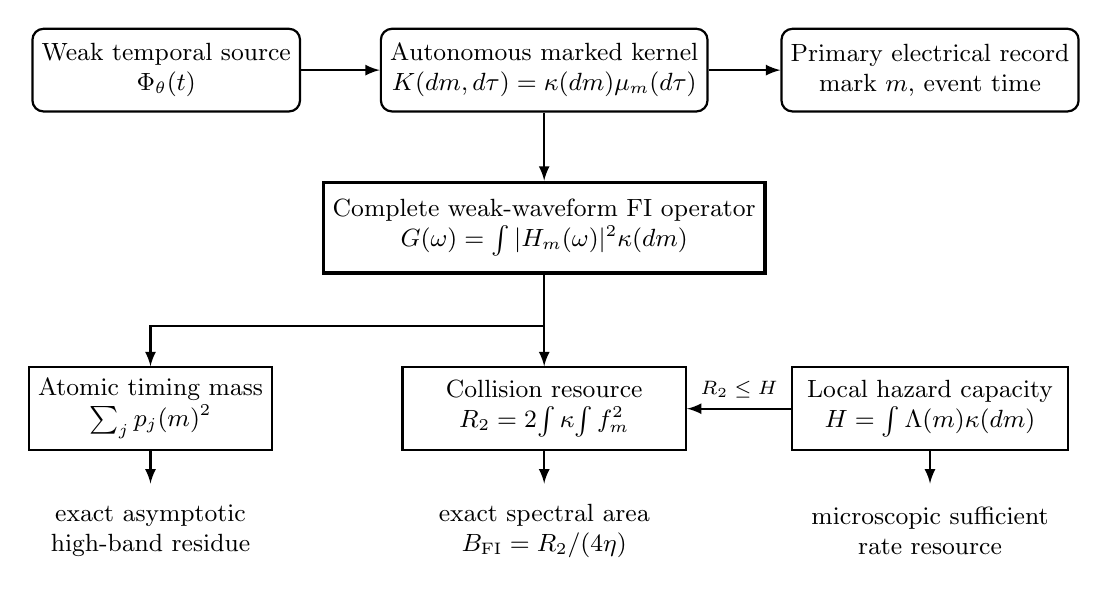
\begin{tikzpicture}[>=latex, line width=0.8pt, font=\small]
  \node[draw, rounded corners, minimum width=3.3cm, minimum height=1.05cm, align=center] (src) at (0,0)
    {Weak temporal source\\$\Phi_{\boldsymbol\theta}(t)$};
  \node[draw, rounded corners, minimum width=4.0cm, minimum height=1.05cm, align=center] (ker) at (4.8,0)
    {Autonomous marked kernel\\$K(dm,d\tau)=\kappa(dm)\mu_m(d\tau)$};
  \node[draw, rounded corners, minimum width=3.5cm, minimum height=1.05cm, align=center] (rec) at (9.7,0)
    {Primary electrical record\\mark $m$, event time};

  \draw[->] (src) -- (ker);
  \draw[->] (ker) -- (rec);

  \node[draw, very thick, minimum width=4.4cm, minimum height=1.15cm, align=center] (G) at (4.8,-2.0)
    {Complete weak-waveform FI operator\\$G(\omega)=\int |H_m(\omega)|^2\kappa(dm)$};
  \draw[->] (ker.south) -- (G.north);

  \node[draw, minimum width=3.0cm, minimum height=1.05cm, align=center] (atom) at (-0.2,-4.3)
    {Atomic timing mass\\$\sum_jp_j(m)^2$};
  \node[draw, minimum width=3.6cm, minimum height=1.05cm, align=center] (r2) at (4.8,-4.3)
    {Collision resource\\$\mathfrak R_2=2\!\int\kappa\!\int f_m^2$};
  \node[draw, minimum width=3.5cm, minimum height=1.05cm, align=center] (haz) at (9.7,-4.3)
    {Local hazard capacity\\$\mathfrak H=\int\Lambda(m)\kappa(dm)$};

  \draw[->] (G.south) -- ++(0,-0.65) -| (atom.north);
  \draw[->] (G.south) -- (r2.north);
  \draw[->] (haz.west) -- node[midway,above,font=\scriptsize] {$\mathfrak R_2\le\mathfrak H$} (r2.east);

  \node[align=center] at (-0.2,-5.85)
    {exact asymptotic\\high-band residue};
  \node[align=center] at (4.8,-5.85)
    {exact spectral area\\$B_{\rm FI}=\mathfrak R_2/(4\eta)$};
  \node[align=center] at (9.7,-5.85)
    {microscopic sufficient\\rate resource};

  \draw[->] (atom.south) -- (-0.2,-5.25);
  \draw[->] (r2.south) -- (4.8,-5.25);
  \draw[->] (haz.south) -- (9.7,-5.25);
\end{tikzpicture}%
}
\caption{Information-transfer and resource hierarchy for the autonomous marked-event theorem. The same spectrum $G(\omega)$ that governs sinusoidal modulation is the spectral multiplier of the complete local weak-waveform Fisher operator. Atomic timing mass controls the exact asymptotic flat-band residue; the capture-weighted collision intensity $\mathfrak R_2$ fixes the integrated transfer spectrum and the equivalent Fisher bandwidth $B_{\rm FI}$; and the capture-weighted local hazard capacity $\mathfrak H$ supplies a microscopic sufficient bound. Source-synchronous control remains an external resource outside the autonomous theorem.}
\label{fig:resourceHierarchy}
\end{figure*}
